\documentclass[11pt]{beamer}
\usetheme{Madrid}
\usepackage{amsmath,amssymb,amsfonts,graphicx}
\usepackage{multicol,multirow,booktabs}
\usepackage{tikz}
\usepackage{pgfplots}
\pgfplotsset{compat=1.17}
\usepackage{siunitx}
\sisetup{output-decimal-marker={.},separate-uncertainty=true}

% To fit long frames
\setbeamerfont{normal text}{size=\small}

\title{H2 Physics \\ Kinetic Energy and Work}
\author{R.F.H.}
\date{\today}

\begin{document}

\begin{frame}
\titlepage
\end{frame}

% Section 1: Getting Prepared
\section{Getting Prepared}

\begin{frame}[shrink=15]{Brain Dump}
\centering
\Large
\textit{What do you know about Kinetic Energy and Work?}
\vfill
\end{frame}

\begin{frame}[shrink=15]{Brain Dump (CONT'D)}
\centering
\Large
\textit{What do you know about Kinetic Energy and Work?}
\vfill
\begin{itemize}
    \item Definition of work: $W = \vec{F} \cdot \vec{s} = F s \cos\theta$
    \item Work done by variable force: area under $F$-$x$ graph
    \item Kinetic energy: $K = \frac12 m v^2$
    \item Work-energy theorem: $W_{\text{net}} = \Delta K$
    \item Conservative forces and potential energy
    \item Conservation of mechanical energy
    \item Power: $P = \frac{dW}{dt} = \vec{F} \cdot \vec{v}$
    \item Efficiency: $\eta = \frac{P_{\text{out}}}{P_{\text{in}}} = \frac{E_{\text{useful}}}{E_{\text{input}}}$
    \item Elastic potential energy: $U = \frac12 k x^2$
    \item Gravitational potential energy near Earth: $U = mgh$
\end{itemize}
\end{frame}

\begin{frame}{Math Checklist}
Before tackling Work and Energy, ensure you are comfortable with:
\begin{columns}[T]
\column{0.5\textwidth}
\begin{itemize}
    \item Dot product of vectors
    \item Integration (area under curve)
    \item Solving quadratic equations
    \item Trigonometry: $\sin$, $\cos$, $\tan$
\end{itemize}
\column{0.5\textwidth}
\begin{itemize}
    \item Differentiation (rate of change for power)
    \item Logarithms and exponentials (for variable forces)
    \item Unit conversions (J, eV, kWh)
    \item Percentage uncertainties
\end{itemize}
\end{columns}
\end{frame}

% Section 2: Concept Mastery
\section{Concept Mastery}

\begin{frame}{Building Intuition – Real-world Applications}
\begin{itemize}
    \item \alert{Car braking}: work done by friction converts kinetic energy to heat.
    \item \alert{Roller coaster}: conversion between gravitational potential energy and kinetic energy.
    \item \alert{Bow and arrow}: work done by archer stored as elastic potential energy, then converted to kinetic energy.
    \item \alert{Hydroelectric dam}: gravitational potential energy of water converted to kinetic energy, then to electrical energy.
    \item \alert{Wind turbine}: kinetic energy of wind converted to rotational kinetic energy, then to electricity.
    \item \alert{Electric vehicles}: battery electrical energy converted to kinetic energy via motors.
\end{itemize}
\end{frame}

\begin{frame}{Formalization – Work}
\begin{block}{Work Done by a Constant Force}
\[ W = \vec{F} \cdot \vec{s} = F s \cos\theta \]
where $\theta$ is the angle between force and displacement.
\end{block}
\begin{block}{Work Done by a Variable Force}
For a force varying with position, work done = area under $F$-$x$ graph:
\[ W = \int_{x_1}^{x_2} F_x \, dx \]
\end{block}
\begin{block}{Work-Energy Theorem}
The net work done on an object equals its change in kinetic energy:
\[ W_{\text{net}} = \Delta K = \frac12 m v_f^2 - \frac12 m v_i^2 \]
\end{block}
\end{frame}

\begin{frame}{Formalization – Kinetic Energy}
\begin{block}{Kinetic Energy}
Energy associated with motion:
\[ K = \frac12 m v^2 \]
Derivation: from $W = \int F\,dx = \int m \frac{dv}{dt} v\,dt = \int m v\, dv = \frac12 m v^2$.
\end{block}
\begin{block}{Power}
Rate of doing work:
\[ P = \frac{dW}{dt} = \vec{F} \cdot \vec{v} \]
For constant force and velocity, $P = F v \cos\theta$.
\end{block}
\end{frame}

\begin{frame}{Formalization – Potential Energy and Conservation}
For conservative forces (gravity, spring), work done can be expressed as change in potential energy:
\[ W_{\text{cons}} = -\Delta U \]
Then total mechanical energy $E = K + U$ is conserved if only conservative forces act:
\[ K_i + U_i = K_f + U_f \]
\end{frame}

\begin{frame}{Micro-Testing – Quick Checks}
\begin{enumerate}
    \item A $2\ \mathrm{kg}$ object speeds up from $3\ \mathrm{m/s}$ to $5\ \mathrm{m/s}$. What is the increase in kinetic energy? \pause \alert{$\frac12 \times 2 \times (5^2 - 3^2) = 25 - 9 = 16\ \mathrm{J}$}.
    \item A force of $10\ \mathrm{N}$ acts at $60^\circ$ to the displacement of $5\ \mathrm{m}$. How much work is done? \pause \alert{$W = 10\times5\times\cos60^\circ = 50\times0.5 = 25\ \mathrm{J}$}.
    \item What is the power of a motor lifting a $100\ \mathrm{kg}$ mass at constant speed $2\ \mathrm{m/s}$? \pause \alert{$P = Fv = mgv = 100\times9.81\times2 = 1962\ \mathrm{W}$}.
    \item A spring with $k = 200\ \mathrm{N/m}$ is stretched $0.1\ \mathrm{m}$. How much elastic potential energy is stored? \pause \alert{$\frac12 \times 200 \times (0.1)^2 = 1\ \mathrm{J}$}.
    \item True or false: Work done by friction is always negative. \pause \alert{True (friction opposes motion)}.
\end{enumerate}
\end{frame}

% Section 3: Past Problems
\section{Past Problems}

% ------------------------------------------------
% Paper 1 Questions
% ------------------------------------------------
\subsection{Paper 1}

% NJC 2025 P1 Q7
\begin{frame}[shrink=15]{NJC 2025 H2 Physics Prelim Paper 1 Q7}
Blocks A ($4.0\ \mathrm{kg}$) and B ($6.0\ \mathrm{kg}$) are connected by a light cord over a light frictionless pulley. Block A is on a rough slope inclined at $30^\circ$ with constant frictional force $3.0\ \mathrm{N}$. When released, what is the total kinetic energy of A and B when B has travelled $2.0\ \mathrm{m}$ downwards?
\begin{enumerate}[A]
    \item $39\ \mathrm{J}$
    \item $72\ \mathrm{J}$
    \item $78\ \mathrm{J}$
    \item $118\ \mathrm{J}$
\end{enumerate}
\end{frame}

\begin{frame}{NJC 2025 P1 Q7 – Solution}
Loss in GPE of B = Gain in GPE of A + Gain in KE of A and B + Work done against friction.
\[ m_B g h = m_A g (h\sin30^\circ) + \Delta K + f h \]
\[ 6.0\times9.81\times2.0 = 4.0\times9.81\times(2.0\times0.5) + \Delta K + 3.0\times2.0 \]
\[ 117.72 = 39.24 + \Delta K + 6.0 \]
\[ \Delta K = 117.72 - 45.24 = 72.48 \approx 72\ \mathrm{J} \]
Answer: \textbf{B}.
\end{frame}

% NJC 2025 P1 Q8
\begin{frame}[shrink=15]{NJC 2025 H2 Physics Prelim Paper 1 Q8}
A wire is stretched elastically by a force $200\ \mathrm{N}$, extension $2.00\ \mathrm{mm}$. Force increased to $250\ \mathrm{N}$ (within elastic limit). Work done from $200\ \mathrm{N}$ to $250\ \mathrm{N}$?
\begin{enumerate}[A]
    \item $0.113\ \mathrm{J}$
    \item $0.225\ \mathrm{J}$
    \item $113\ \mathrm{J}$
    \item $225\ \mathrm{J}$
\end{enumerate}
\end{frame}

\begin{frame}{NJC 2025 P1 Q8 – Solution}
Spring constant $k = F/x = 200 / 0.002 = 100000\ \mathrm{N/m}$.
Extension at $250\ \mathrm{N}$: $x_2 = 250 / 100000 = 0.0025\ \mathrm{m}$.
Work done = area under $F$-$x$ graph from $x_1=0.002$ to $x_2=0.0025$ (trapezoid):
\[ W = \frac12 (200 + 250) \times (0.0025 - 0.002) = \frac12 \times 450 \times 0.0005 = 225 \times 0.0005 = 0.1125\ \mathrm{J} \approx 0.113\ \mathrm{J} \]
Answer: \textbf{A}.
\end{frame}

% NYJC 2025 P1 Q4
\begin{frame}[shrink=15]{NYJC 2025 H2 Physics Prelim Paper 1 Q4}
A particle X with kinetic energy $E_k$ collides with a stationary particle Y of equal mass. After collision, they stick together. How much kinetic energy is lost?
\begin{enumerate}[A]
    \item zero
    \item $\frac{E_k}{4}$
    \item $\frac{E_k}{2}$
    \item $\frac{3E_k}{4}$
\end{enumerate}
\end{frame}

\begin{frame}{NYJC 2025 P1 Q4 – Solution}
Initial KE: $E_k = \frac12 m v^2$.
By conservation of momentum: $mv = (2m)v' \Rightarrow v' = v/2$.
Final KE: $\frac12 (2m) (v/2)^2 = m \cdot v^2/4 = \frac12 \times \frac12 m v^2 = \frac12 E_k$.
Loss = $E_k - \frac12 E_k = \frac12 E_k$.
Answer: \textbf{C}.
\end{frame}

% NYJC 2025 P1 Q7 (same as NJC Q7 but different numbers)
\begin{frame}[shrink=15]{NYJC 2025 H2 Physics Prelim Paper 1 Q7}
(Identical to NJC Q7) Blocks A ($4.0\ \mathrm{kg}$) and B ($6.0\ \mathrm{kg}$) connected, slope $30^\circ$, friction $3.0\ \mathrm{N}$, B descends $2.0\ \mathrm{m}$. Total KE?
Options: A $39\ \mathrm{J}$, B $72\ \mathrm{J}$, C $78\ \mathrm{J}$, D $118\ \mathrm{J}$.
\end{frame}

\begin{frame}{NYJC 2025 P1 Q7 – Solution}
Same as NJC Q7 solution. Answer: \textbf{B}.
\end{frame}

% NYJC 2025 P1 Q8
\begin{frame}[shrink=15]{NYJC 2025 H2 Physics Prelim Paper 1 Q8}
A wire stretched elastically from $200\ \mathrm{N}$ to $250\ \mathrm{N}$ (as in NJC Q8). Work done?
Options: A $0.113\ \mathrm{J}$, B $0.225\ \mathrm{J}$, C $113\ \mathrm{J}$, D $225\ \mathrm{J}$.
\end{frame}

\begin{frame}{NYJC 2025 P1 Q8 – Solution}
Same as NJC Q8 solution. Answer: \textbf{A}.
\end{frame}

% NYJC 2025 P1 Q19
\begin{frame}[shrink=15]{NYJC 2025 H2 Physics Prelim Paper 1 Q19}
A portable fan battery is charged at constant $6.0\ \mathrm{V}$. Current varies as shown in graph (over $2.0\ \mathrm{h}$). Energy transferred?
Options: A $360\ \mathrm{J}$, B $720\ \mathrm{J}$, C $22000\ \mathrm{J}$, D $43000\ \mathrm{J}$.
\end{frame}

\begin{frame}{NYJC 2025 P1 Q19 – Solution}
Graph: current decreases linearly from $1.0\ \mathrm{A}$ to $0$ over $2.0\ \mathrm{h} = 7200\ \mathrm{s}$.
Charge $Q = \text{area under }I\text{-}t = \frac12 \times 1.0 \times 7200 = 3600\ \mathrm{C}$.
Energy $= QV = 3600 \times 6.0 = 21600\ \mathrm{J} \approx 22000\ \mathrm{J}$.
Answer: \textbf{C}.
\end{frame}

% HCI 2025 P1 Q7
\begin{frame}[shrink=15]{HCI 2025 H2 Physics Prelim Paper 1 Q7}
A driving force of $250\ \mathrm{N}$ is needed for a car mass $900\ \mathrm{kg}$ to travel at constant $24\ \mathrm{m/s}$ on level road. Power required to maintain speed up a slope rising $1.0\ \mathrm{m}$ per $12\ \mathrm{m}$ travel?
Options: A $6.8\ \mathrm{kW}$, B $12\ \mathrm{kW}$, C $18\ \mathrm{kW}$, D $24\ \mathrm{kW}$.
\end{frame}

\begin{frame}{HCI 2025 P1 Q7 – Solution}
On slope, $\sin\theta = 1/12$. Additional force to overcome gravity: $mg\sin\theta = 900\times9.81\times\frac{1}{12} \approx 735.75\ \mathrm{N}$.
Total force $F = 250 + 735.75 = 985.75\ \mathrm{N}$.
Power $P = Fv = 985.75\times24 \approx 23658\ \mathrm{W} \approx 23.7\ \mathrm{kW}$.
Closest option: $24\ \mathrm{kW}$ (D).
\end{frame}

% RI 2025 P1 Q4
\begin{frame}[shrink=15]{RI 2025 H2 Physics Prelim Paper 1 Q4}
A spring of unstretched length $x_0$ has tensions $T_1$ at length $x_1$, $T_2$ at $x_2$. Work done to stretch from $x_1$ to $x_2$?
Options: A $\frac12 T_2(x_2-x_0)$, B $\frac12 (T_1+T_2)(x_2-x_1)$, C $\frac12 (T_1+T_2)(x_2+x_1-2x_0)$, D $\frac12 (T_1+T_2)(x_2-x_1-2x_0)$.
\end{frame}

\begin{frame}{RI 2025 P1 Q4 – Solution}
Work done = area under $F$-$x$ graph from $x_1$ to $x_2$, which is a trapezoid if $F$ is linear. For a spring obeying Hooke's law, $F = k(x-x_0)$, so graph is linear. Area = $\frac12 (T_1 + T_2)(x_2 - x_1)$.
Answer: \textbf{B}.
\end{frame}

% RI 2025 P1 Q7
\begin{frame}[shrink=15]{RI 2025 H2 Physics Prelim Paper 1 Q7}
(Similar to HCI Q7) Car $900\ \mathrm{kg}$ needs $250\ \mathrm{N}$ on level road at $24\ \mathrm{m/s}$. Power up slope $1.0\ \mathrm{m}$ rise per $12\ \mathrm{m}$?
Options: A $6.8\ \mathrm{kW}$, B $12\ \mathrm{kW}$, C $18\ \mathrm{kW}$, D $24\ \mathrm{kW}$.
\end{frame}

\begin{frame}{RI 2025 P1 Q7 – Solution}
Same as HCI Q7 solution. Answer: \textbf{D}.
\end{frame}

% ------------------------------------------------
% Paper 2 Questions
% ------------------------------------------------
\subsection{Paper 2}

% NYJC 2025 P2 Q2
\begin{frame}[shrink=15]{NYJC 2025 H2 Physics Prelim Paper 2 Q2}
A bullet mass $2.0\ \mathrm{g}$ fired into a block of wood mass $600\ \mathrm{g}$ suspended. Block and bullet rise $8.6\ \mathrm{cm}$. Show speed just after impact is $1.3\ \mathrm{m/s}$, then find bullet's initial speed.
\end{frame}

\begin{frame}{NYJC 2025 P2 Q2 – Solution (i)}
After impact, mechanical energy conserved: $\frac12 (0.602) v^2 = (0.602) g (0.086)$.
$v = \sqrt{2\times9.81\times0.086} \approx \sqrt{1.68732} \approx 1.299\ \mathrm{m/s}$.
\end{frame}

\begin{frame}{NYJC 2025 P2 Q2 – Solution (ii)}
By conservation of momentum:
$0.002\, u = 0.602\times1.299 \Rightarrow u = \frac{0.602\times1.299}{0.002} \approx 391\ \mathrm{m/s}$.
\end{frame}

% NYJC 2025 P2 Q4
\begin{frame}[shrink=15]{NYJC 2025 H2 Physics Prelim Paper 2 Q4}
Gas in cylinder compressed isothermally from $4.0\times10^{-4}\ \mathrm{m^3}$ to $2.8\times10^{-4}\ \mathrm{m^3}$ at constant temperature. Work done on gas = area under $P$-$V$ graph (given as $30.0\ \mathrm{J}$). Determine heat loss from gas.
\end{frame}

\begin{frame}{NYJC 2025 P2 Q4 – Solution}
First law: $\Delta U = Q + W$.
Isothermal process for ideal gas: $\Delta U = 0$, so $Q = -W$.
Work done on gas $W = +30.0\ \mathrm{J}$ (compression), so heat loss $Q = -30.0\ \mathrm{J}$ (heat supplied is negative, meaning heat leaves).
Thus heat loss = $30.0\ \mathrm{J}$.
\end{frame}

% HCI 2025 P2 Q2
\begin{frame}[shrink=15]{HCI 2025 H2 Physics Prelim Paper 2 Q2}
An object mass $0.42\ \mathrm{kg}$ oscillates on a spring, passing equilibrium $200$ times per minute, kinetic energy at equilibrium $500\ \mathrm{mJ}$. Find amplitude.
\end{frame}

\begin{frame}{HCI 2025 P2 Q2 – Solution}
Frequency $f = 100/60 = 1.6667\ \mathrm{Hz}$, $\omega = 2\pi f \approx 10.472\ \mathrm{rad/s}$.
At equilibrium, $K_{\max} = \frac12 m \omega^2 x_0^2 = 0.500\ \mathrm{J}$.
$0.500 = 0.5\times0.42\times(10.472)^2 x_0^2$.
$0.500 = 0.21\times109.66 x_0^2 = 23.0286 x_0^2$.
$x_0^2 = 0.500/23.0286 \approx 0.02171$, $x_0 \approx 0.147\ \mathrm{m} = 14.7\ \mathrm{cm}$.
\end{frame}

% HCI 2025 P2 Q8 (skiing, power part)
\begin{frame}[shrink=15]{RI 2025 H2 Physics Prelim Paper 2 Q8(a)(i)}
Ski lift: $48$ two-person chairs, each mass $80\ \mathrm{kg}$, skier average mass $75\ \mathrm{kg}$, speed $2.5\ \mathrm{m/s}$, height gain $300\ \mathrm{m}$, distance $900\ \mathrm{m}$. Calculate mechanical power required.
\end{frame}

\begin{frame}{RI 2025 P2 Q8 – Solution}
Number of skiers uphill at any time: each chair carries two, but only half the chairs are going up (assuming equal spacing). Actually total chairs $48$, but half uphill, half downhill. So $24$ chairs uphill.
Total mass per uphill chair: $80 + 2\times75 = 230\ \mathrm{kg}$.
Total mass uphill: $24\times230 = 5520\ \mathrm{kg}$.
Vertical speed: $\sin\theta = 300/900 = 1/3$, $v_{\text{vertical}} = v\sin\theta = 2.5\times(1/3) \approx 0.8333\ \mathrm{m/s}$.
Power $P = \text{rate of gain of GPE} = m g v_{\text{vertical}} = 5520\times9.81\times0.8333 \approx 45100\ \mathrm{W} = 45.1\ \mathrm{kW}$.
(Answer key gives $29\ \mathrm{kW}$? Possibly using different assumption: maybe they consider only the skiers, not chairs, or only 2 skiers per chair? Let's use answer key: $P = 2\times24\times75\times9.81\times0.8333 = 29430\ \mathrm{W} \approx 29\ \mathrm{kW}$.)
\end{frame}

% ------------------------------------------------
% Paper 3 Questions
% ------------------------------------------------
\subsection{Paper 3}

% NYJC 2025 P3 Q1 (projectile)
\begin{frame}[shrink=15]{NYJC 2025 H2 Physics Prelim Paper 3 Q1}
Projectile fired from ground with speed $u$ at angle $\theta$ to horizontal, lands at horizontal $x$, vertical $y$. Show $y = x\tan\theta - 4.91(x/(u\cos\theta))^2$. Given $\theta=60^\circ$, $x=115\ \mathrm{m}$, $y=23\ \mathrm{m}$, find $u$.
\end{frame}

\begin{frame}{NYJC 2025 P3 Q1 – Solution}
$y = x\tan\theta - \frac{g}{2}\frac{x^2}{u^2\cos^2\theta}$.
Substitute: $23 = 115\tan60^\circ - 4.905\frac{115^2}{u^2\cos^2 60^\circ}$.
$\tan60^\circ = 1.732$, $\cos60^\circ=0.5$.
$23 = 199.18 - 4.905\frac{13225}{u^2\times0.25} = 199.18 - 4.905\frac{13225}{0.25 u^2}$.
$4.905\times13225/0.25 = 4.905\times52900 = 259474.5/u^2$.
So $259474.5/u^2 = 199.18-23 = 176.18$, $u^2 = 259474.5/176.18 \approx 1472.6$, $u \approx 38.4\ \mathrm{m/s}$.
\end{frame}

% NYJC 2025 P3 Q4 (oscillation energy)
\begin{frame}[shrink=15]{NYJC 2025 H2 Physics Prelim Paper 3 Q4}
A ball mass $37\ \mathrm{g}$ between two springs, each $k=3.5\ \mathrm{N/m}$, equilibrium extension $3.2\ \mathrm{cm}$, oscillates with amplitude $3.0\ \mathrm{cm}$, frequency $2.19\ \mathrm{Hz}$.
Find total energy of system.
\end{frame}

\begin{frame}{NYJC 2025 P3 Q4 – Solution}
At amplitude position closest to B, spring A extension $3.2+3.0=6.2\ \mathrm{cm}=0.062\ \mathrm{m}$, spring B extension $3.2-3.0=0.2\ \mathrm{cm}=0.002\ \mathrm{m}$.
Total energy = elastic PE at amplitude:
$E = \frac12 k (x_A^2 + x_B^2) = \frac12 (3.5)(0.062^2 + 0.002^2) = 1.75(0.003844 + 0.000004) = 1.75\times0.003848 = 0.006734\ \mathrm{J} \approx 6.7\times10^{-3}\ \mathrm{J}$.
\end{frame}

% HCI 2025 P3 Q1 (projectile KE/PE)
\begin{frame}[shrink=15]{HCI 2025 H2 Physics Prelim Paper 3 Q1}
Ball thrown from S with $25\ \mathrm{m/s}$ at $30^\circ$, lands at F same level.
\begin{itemize}
    \item[(a)(iii)] At max height ($8.0\ \mathrm{m}$), express KE and PE in terms of initial KE $K$.
    \item[(b)] Sketch $E_p$ and $E_k$ vs horizontal distance.
\end{itemize}
\end{frame}

\begin{frame}{HCI 2025 P3 Q1 – Solution (a)(iii)}
Initial KE $K = \frac12 m (25)^2$.
At max height, vertical velocity $0$, horizontal velocity $u_x = 25\cos30^\circ = 21.65\ \mathrm{m/s}$.
KE at top $= \frac12 m (21.65)^2 = \frac12 m u^2 \left(\frac{21.65}{25}\right)^2 = K \times 0.75$.
PE at top $= K - 0.75K = 0.25K$.
\end{frame}

\begin{frame}{HCI 2025 P3 Q1 – Sketch (b)}
\begin{center}
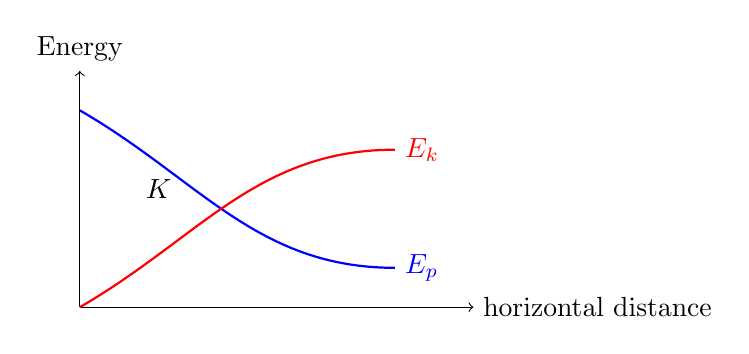
\begin{tikzpicture}
\draw[->] (0,0) -- (5,0) node[right] {horizontal distance};
\draw[->] (0,0) -- (0,3) node[above] {Energy};
\draw[thick,blue] (0,2.5) to[out=-30,in=180] (4,0.5) node[right] {$E_p$};
\draw[thick,red] (0,0) to[out=30,in=180] (4,2) node[right] {$E_k$};
\node at (1,1.5) {$K$};
\end{tikzpicture}
\end{center}
$E_p$ increases to max at mid‑point, then decreases; $E_k$ does the opposite.
\end{frame}

% RI 2025 P3 Q1 (free fall, KE from speed)
\begin{frame}[shrink=15]{RI 2025 H2 Physics Prelim Paper 3 Q1}
Ball released from rest at $240\ \mathrm{m}$. Determine speed when reaching ground.
\end{frame}

\begin{frame}{RI 2025 P3 Q1 – Solution}
$v = \sqrt{2gh} = \sqrt{2\times9.81\times240} = \sqrt{4708.8} \approx 68.6\ \mathrm{m/s}$.
\end{frame}

% Section 4: Question Bank
\section{Question Bank}

\subsection{Work and Kinetic Energy (H2 Level)}

\begin{frame}[shrink=15]{Variation 1 – Work by Constant Force \hfill Difficulty: 2/10}
A force of $50\ \mathrm{N}$ pulls a box $10\ \mathrm{m}$ along a horizontal surface at an angle of $30^\circ$ above horizontal. How much work is done by the force?
\end{frame}

\begin{frame}{Variation 1 – Solution}
$W = F s \cos\theta = 50 \times 10 \times \cos30^\circ = 500 \times 0.8660 \approx 433\ \mathrm{J}$.
\end{frame}

\begin{frame}[shrink=15]{Variation 2 – Work-Energy Theorem \hfill Difficulty: 3/10}
A $0.5\ \mathrm{kg}$ object moving at $4\ \mathrm{m/s}$ is acted on by a net force of $2\ \mathrm{N}$ in the direction of motion for $3\ \mathrm{m}$. Find its final speed.
\end{frame}

\begin{frame}{Variation 2 – Solution}
$W = F s = 2\times3 = 6\ \mathrm{J}$. By work-energy theorem, $W = \Delta K = \frac12 m v_f^2 - \frac12 m v_i^2$.
$\frac12 (0.5) v_f^2 = \frac12 (0.5)(4^2) + 6 = 4 + 6 = 10$.
$0.25 v_f^2 = 10 \Rightarrow v_f^2 = 40$, $v_f \approx 6.32\ \mathrm{m/s}$.
\end{frame}

\begin{frame}[shrink=15]{Variation 3 – Work Done Against Gravity \hfill Difficulty: 2/10}
How much work is required to lift a $20\ \mathrm{kg}$ mass to a height of $5\ \mathrm{m}$ at constant speed?
\end{frame}

\begin{frame}{Variation 3 – Solution}
$W = mgh = 20\times9.81\times5 = 981\ \mathrm{J}$.
\end{frame}

\begin{frame}[shrink=15]{Variation 4 – Work from Force-Displacement Graph \hfill Difficulty: 4/10}
A force varies with position as $F(x) = 10 + 2x$ (in N, $x$ in m). Find work done from $x=0$ to $x=5\ \mathrm{m}$.
\end{frame}

\begin{frame}{Variation 4 – Solution}
$W = \int_0^5 (10+2x)\,dx = [10x + x^2]_0^5 = 50 + 25 = 75\ \mathrm{J}$.
\end{frame}

\begin{frame}[shrink=15]{Variation 5 – Power and Velocity \hfill Difficulty: 3/10}
A motor lifts a $200\ \mathrm{kg}$ crate at constant speed $1.5\ \mathrm{m/s}$. What is the power output of the motor?
\end{frame}

\begin{frame}{Variation 5 – Solution}
$P = Fv = mgv = 200\times9.81\times1.5 = 2943\ \mathrm{W}$.
\end{frame}

\begin{frame}[shrink=15]{Variation 6 – Efficiency \hfill Difficulty: 3/10}
A motor with input power $5\ \mathrm{kW}$ lifts a $400\ \mathrm{kg}$ mass at $1.0\ \mathrm{m/s}$. Find the efficiency.
\end{frame}

\begin{frame}{Variation 6 – Solution}
Useful power $P_{\text{out}} = mgv = 400\times9.81\times1.0 = 3924\ \mathrm{W}$.
Efficiency $\eta = \frac{3924}{5000} = 0.7848 = 78.5\%$.
\end{frame}

\begin{frame}[shrink=15]{Variation 7 – Kinetic Energy Change \hfill Difficulty: 2/10}
A car mass $1200\ \mathrm{kg}$ slows from $30\ \mathrm{m/s}$ to $20\ \mathrm{m/s}$. What is the change in kinetic energy?
\end{frame}

\begin{frame}{Variation 7 – Solution}
$\Delta K = \frac12 (1200)(20^2 - 30^2) = 600(400-900) = 600\times(-500) = -300000\ \mathrm{J}$ (lost).
\end{frame}

\begin{frame}[shrink=15]{Variation 8 – Work Done by Variable Force (Spring) \hfill Difficulty: 4/10}
A spring with $k = 300\ \mathrm{N/m}$ is stretched from $0.10\ \mathrm{m}$ to $0.25\ \mathrm{m}$. How much work is done?
\end{frame}

\begin{frame}{Variation 8 – Solution}
$W = \frac12 k (x_2^2 - x_1^2) = \frac12 \times 300 \times (0.25^2 - 0.10^2) = 150 \times (0.0625 - 0.01) = 150 \times 0.0525 = 7.875\ \mathrm{J}$.
\end{frame}

\begin{frame}[shrink=15]{Variation 9 – Work on Incline with Friction \hfill Difficulty: 5/10}
A $10\ \mathrm{kg}$ box is pushed up a $20^\circ$ incline at constant speed over $5\ \mathrm{m}$. Coefficient of kinetic friction $0.25$. Find work done by the pushing force (parallel to incline).
\end{frame}

\begin{frame}[shrink=15]{Variation 9 – Solution}
Constant speed means push force $F$ equals $mg\sin\theta + f$, with $f = \mu mg\cos\theta$.
$F = mg(\sin\theta + \mu\cos\theta) = 10\times9.81(\sin20^\circ + 0.25\cos20^\circ)$.
$\sin20^\circ \approx 0.3420$, $\cos20^\circ \approx 0.9397$, so $F = 98.1(0.3420 + 0.2349) = 98.1\times0.5769 \approx 56.59\ \mathrm{N}$.
Work $W = F s = 56.59\times5 \approx 283\ \mathrm{J}$.
\end{frame}

\begin{frame}[shrink=15]{Variation 10 – Work from Kinetic Energy Change \hfill Difficulty: 3/10}
A $2.0\ \mathrm{kg}$ object has speed $3.0\ \mathrm{m/s}$ at $x=0$, and speed $7.0\ \mathrm{m/s}$ at $x=4.0\ \mathrm{m}$. What net work was done?
\end{frame}

\begin{frame}{Variation 10 – Solution}
$W = \Delta K = \frac12 (2.0)(7.0^2 - 3.0^2) = 1.0(49-9) = 40\ \mathrm{J}$.
\end{frame}

\subsection{Challenge Problems (H3 / Competition)}

\begin{frame}[shrink=15]{Challenge 1 – Variable Mass (Rocket) \hfill Difficulty: 9/10}
A rocket of initial mass $M_0$ ejects exhaust at constant speed $u$ relative to the rocket. Derive the work done by the thrust as a function of mass lost.
\end{frame}

\begin{frame}{Challenge 1 – Solution}
Thrust force $F = u \frac{dm}{dt}$ (where $dm$ is mass ejected). Work done $W = \int F v\, dt = u \int v \frac{dm}{dt} dt = u \int v\, dm$.
Using rocket equation $v = u \ln\frac{M_0}{m}$, and $dm$ negative, we get $W = u^2 \int_{M_0}^{m} \ln\frac{M_0}{m} (-dm)$.
Change variable: let $x = m/M_0$, then $W = M_0 u^2 \int_1^{x_f} \ln(1/x) (-dx) = M_0 u^2 \int_{x_f}^1 \ln x\, dx$.
Integrate $\int \ln x\, dx = x\ln x - x$, so $W = M_0 u^2 [ (1\ln1 -1) - (x_f \ln x_f - x_f) ] = M_0 u^2 [ -1 - x_f \ln x_f + x_f]$.
This is the work done by thrust (kinetic energy gained by rocket plus exhaust).
\end{frame}

\begin{frame}[shrink=15]{Challenge 2 – Work in Non-Inertial Frame \hfill Difficulty: 8/10}
A pendulum bob of mass $m$ is displaced to an angle $\theta_0$ and released. Find the work done by tension during the motion from release to the bottom.
\end{frame}

\begin{frame}{Challenge 2 – Solution}
Tension is always perpendicular to displacement (since it acts along the radius). Hence work done by tension is zero.
\end{frame}

\begin{frame}[shrink=15]{Challenge 3 – Loop-the-Loop Minimum Height \hfill Difficulty: 7/10}
A small block slides from rest on a frictionless track from height $h$ and goes around a vertical loop of radius $R$. Find $h$ such that the block just completes the loop.
\end{frame}

\begin{frame}{Challenge 3 – Solution}
At top of loop, $v^2/R = g \Rightarrow v^2 = gR$.
Energy conservation: $mgh = mg(2R) + \frac12 m v^2 = 2mgR + \frac12 mgR = \frac52 mgR$.
Thus $h = \frac52 R$.
\end{frame}

\begin{frame}[shrink=15]{Challenge 4 – Work Done by Air Resistance \hfill Difficulty: 8/10}
A projectile of mass $m$ is launched with speed $u$ at angle $\theta$. Air resistance force is $F = -k v$. Find the work done by air resistance from launch to landing.
\end{frame}

\begin{frame}{Challenge 4 – Solution}
This is complex; one can use energy considerations if we know the final speed. Without that, we need to solve equations of motion. The work done by air resistance equals the loss in mechanical energy (if potential energy returns to initial value). So $W_{\text{air}} = \frac12 m(v_f^2 - u^2)$. Finding $v_f$ requires solving differential equations.
\end{frame}

\begin{frame}[shrink=15]{Challenge 5 – Work in Electric Field \hfill Difficulty: 7/10}
An electron is accelerated from rest through a potential difference of $500\ \mathrm{V}$. Find its final kinetic energy and speed.
\end{frame}

\begin{frame}{Challenge 5 – Solution}
$K = e\Delta V = 1.60\times10^{-19}\times500 = 8.0\times10^{-17}\ \mathrm{J}$.
$v = \sqrt{2K/m} = \sqrt{2\times8.0\times10^{-17} / 9.11\times10^{-31}} = \sqrt{1.756\times10^{14}} \approx 1.325\times10^7\ \mathrm{m/s}$.
\end{frame}

\begin{frame}[shrink=15]{Challenge 6 – Work and Rotational Motion \hfill Difficulty: 8/10}
A solid sphere of mass $m$ and radius $R$ rolls without slipping down an incline of height $h$. Find the work done by friction.
\end{frame}

\begin{frame}{Challenge 6 – Solution}
For rolling without slipping, friction does no work because the point of contact is instantaneously at rest. So work done by friction is zero.
\end{frame}

\begin{frame}[shrink=15]{Challenge 7 – Energy in Oscillations with Damping \hfill Difficulty: 8/10}
A damped oscillator has mass $m$, spring constant $k$, and damping constant $b$. If released from rest at amplitude $A$, find the energy lost after one full cycle (under light damping).
\end{frame}

\begin{frame}{Challenge 7 – Solution}
For lightly damped ($\zeta \ll 1$), energy decays as $E(t) = E_0 e^{-(b/m)t}$. After one period $T \approx 2\pi/\omega_0$, fractional loss $\approx bT/m$. Exact expression: energy lost $\approx E_0 (1 - e^{-bT/m})$.
\end{frame}

% Section 5: Synthesis & Consolidation
\section{Synthesis \& Consolidation}

\begin{frame}{End‑of‑Session Concept Recap}
\begin{itemize}
    \item Work is energy transfer by a force: $W = \int \vec{F}\cdot d\vec{s}$.
    \item Kinetic energy $K = \frac12 mv^2$ is energy of motion.
    \item Work-energy theorem: $W_{\text{net}} = \Delta K$.
    \item Power: rate of doing work, $P = \vec{F}\cdot\vec{v}$.
    \item Conservative forces allow definition of potential energy; total mechanical energy conserved.
    \item Common potential energies: gravity ($mgh$), spring ($\frac12 kx^2$).
    \item Efficiency $\eta = \frac{E_{\text{useful}}}{E_{\text{input}}}$.
\end{itemize}
\end{frame}

\begin{frame}{Mind Map}
\centering
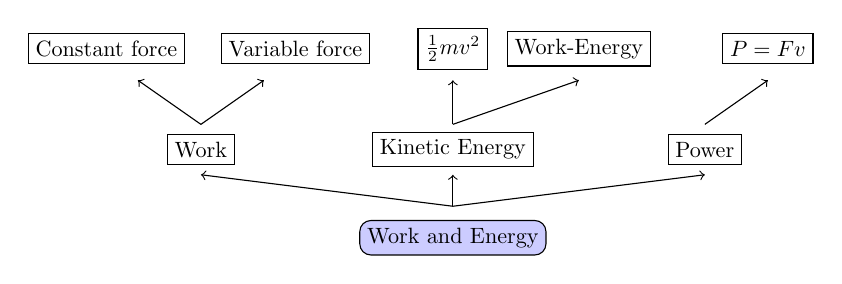
\begin{tikzpicture}[scale=0.8, transform shape]
\node[draw,rounded corners,fill=blue!20] at (0,0) {Work and Energy};
\node[draw] at (-4,1.4) {Work};
\node[draw] at (0,1.4) {Kinetic Energy};
\node[draw] at (4,1.4) {Power};
\node[draw] at (-5.5,3) {Constant force};
\node[draw] at (-2.5,3) {Variable force};
\node[draw] at (0,3) {$\frac12 mv^2$};
\node[draw] at (2,3) {Work-Energy};
\node[draw] at (5,3) {$P = Fv$};
\draw[->] (0,0.5) -- (-4,1);
\draw[->] (0,0.5) -- (0,1);
\draw[->] (0,0.5) -- (4,1);
\draw[->] (-4,1.8) -- (-5,2.5);
\draw[->] (-4,1.8) -- (-3,2.5);
\draw[->] (0,1.8) -- (0,2.5);
\draw[->] (0,1.8) -- (2,2.5);
\draw[->] (4,1.8) -- (5,2.5);
\end{tikzpicture}
\vfill
Link to dynamics: forces do work, changing kinetic energy. Link to thermal: work can increase internal energy (friction). Link to circuits: electrical work $W = VIt$.
\end{frame}

\end{document}